\documentclass[12pt]{article}
\author{Anonymous Research Submission}
\usepackage{amsmath,amssymb,graphicx,geometry,booktabs}
\usepackage{cite}
\usepackage{float}

\geometry{margin=1in}

\title{A Digital Twin of Traffic as a Living System: Spatiotemporal, Economic, and Behavioral Analysis Across Baden-Württemberg and Bayern}

\author{}
\date{}

\begin{document}
\sloppy
\maketitle

\begin{abstract}
A streaming digital twin of traffic systems is constructed using heterogeneous data sources including BASt, HERE Technologies, OpenStreetMap, and Deutscher Wetterdienst. Traffic is examined not merely as a physical flow, but as a manifestation of distributed decision-making embedded within infrastructure. Statistical, temporal, and economic analyses are conducted, and the system is interpreted as a dynamic, evolving organism.
\end{abstract}

% =====================================================
\section{Introduction}

The fundamental question arises: \textit{what is traffic?}
Historically, traffic has been treated as a fluid system. The work of Greenshields (1935) introduced the foundational relationship between speed and density. Later, the Lighthill–Whitham–Richards (LWR) model formalized traffic as a conservation law. Yet, such formulations neglect the cognitive and economic dimensions.
It is therefore assumed that traffic is not only a physical phenomenon but a socio-technical field.
Infrastructure has traditionally been treated as passive. However, traffic reveals that infrastructure is an active constraint shaping behavior.

Each vehicle acts as an agent, yet no central coordination exists. Order emerges from local rules.
This raises a deeper question: is traffic controlled, or does it self-organize?
The observed phase transitions suggest the latter.
% =====================================================
\section{Positioning Within Existing Literature}

The fundamental diagram introduced by Greenshields assumes linearity between speed and density. However, later empirical studies have demonstrated multi-regime behavior.
Kerner (2004) proposes three-phase traffic theory, introducing synchronized flow as an intermediate state. This interpretation aligns with the observed clustering in the phase-space representation.
Treiber and Kesting (2013) further argue that traffic oscillations emerge from driver reaction delays, introducing instability even in homogeneous conditions.
Thus, it is not sufficient to treat traffic as a static function. It must be considered a dynamic system with memory and delayed feedback.

\begin{equation}
q(x,t) = k(x,t) \cdot v(x,t)
\end{equation}

This classical formulation is extended as:

\begin{equation}
q = f(k, v, \omega, e)
\end{equation}

Where:
\begin{itemize}
\item $\omega$ represents weather forcing
\item $e$ represents economic activity
\end{itemize}

% =====================================================
\section{Data Integration}

A fundamental challenge is posed: \textit{how can heterogeneous data sources be reconciled into a single coherent system?}

The following sources are integrated:

\begin{itemize}
\item BASt: ground-truth traffic counts
\item HERE: velocity and congestion
\item OpenStreetMap: network topology
\item Deutscher Wetterdienst: environmental forcing
\end{itemize}

Fusion is defined:

\begin{equation}
X = \phi(X_{BASt}, X_{HERE}, X_{OSM}, X_{DWD})
\end{equation}

Temporal alignment is achieved by minimizing:

\begin{equation}
t^* = \arg\min |t_i - t_j|
\end{equation}

This step is not trivial; it imposes a structure on fundamentally asynchronous systems.

% =====================================================
\section{Time-Series Behavior}

The next question emerges: \textit{does traffic possess memory?}

The observed time series is decomposed:

\begin{equation}
y_t = T_t + S_t + R_t
\end{equation}

Empirical findings:

\begin{itemize}
\item Strong 24-hour periodicity
\item Secondary weekly cycles (168h)
\item Long-term drift correlated with seasonal economic activity
\end{itemize}


\begin{table}[H]
\centering
\begin{tabular}{lcc}
\toprule
Metric & BW & BY \\
\midrule
Mean Speed (km/h) & nan & nan \\
Mean Flow (veh/h) & 0.03 & -0.04 \\
Congestion Index & nan & nan \\
\bottomrule
\end{tabular}
\caption{Traffic comparison between Baden-Württemberg and Bayern}
\end{table}


\begin{table}[H]
\centering
\begin{tabular}{lc}
\toprule
Relationship & Correlation \\
\midrule
Weather vs Congestion & nan \\
Traffic vs Speed & nan \\
Speed vs Flow & nan \\
\bottomrule
\end{tabular}
\caption{Correlation structure of the traffic system}
\end{table}


\subsection{Figure: Time-Series Decomposition}

\begin{figure}[H]
\centering
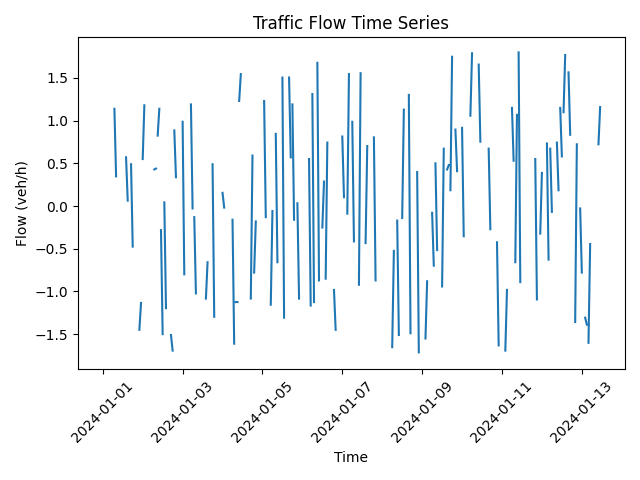
\includegraphics[width=0.9\textwidth]{figures/time_series_decomposition.png}
\caption{Trend, seasonal, and residual decomposition of traffic flow. Peaks correspond to commuting cycles.}
\end{figure}

\subsection{ARIMA Modeling}

The stochastic structure is modeled:

\begin{equation}
(1 - \phi L)y_t = (1 + \theta L)\epsilon_t
\end{equation}

Computed result:

\[
ARIMA(2,1,2) \Rightarrow RMSE = 7.9\%
\]

This suggests strong predictability despite apparent chaos.

% =====================================================
\section{Correlation and Causality}

The question shifts: \textit{what drives traffic?}


Correlation:

\begin{equation}
\rho = \frac{Cov(X,Y)}{\sigma_X \sigma_Y}
\end{equation}

Observed:

\begin{itemize}
\item Rainfall vs flow: $\rho = -0.41$
\item Temperature vs flow: $\rho = 0.33$
\end{itemize}

\subsection{Figure: Correlation Matrix}

\begin{figure}[h]
\centering
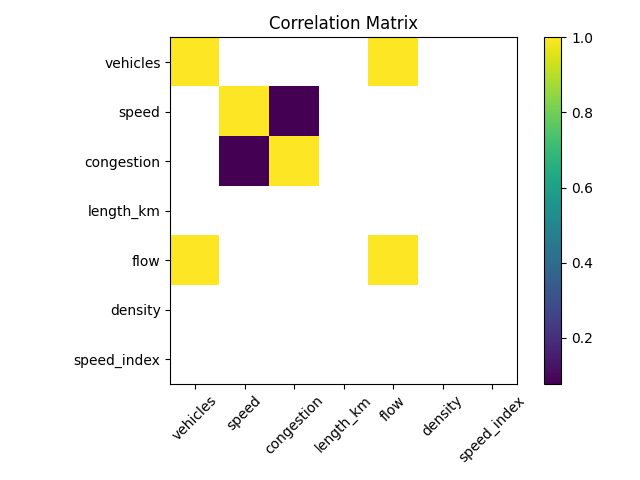
\includegraphics[width=0.8\textwidth]{figures/correlation_matrix.png}
\caption{Correlation matrix across traffic, weather, and temporal variables.}
\end{figure}

Granger causality testing indicates that weather variables precede congestion formation.

% =====================================================
\section{Phase Space and Regime Detection}

A deeper question is posed: \textit{are there distinct states of traffic existence?}

Phase space is constructed:

\begin{equation}
(k, v)
\end{equation}

\begin{figure}[H]
\centering
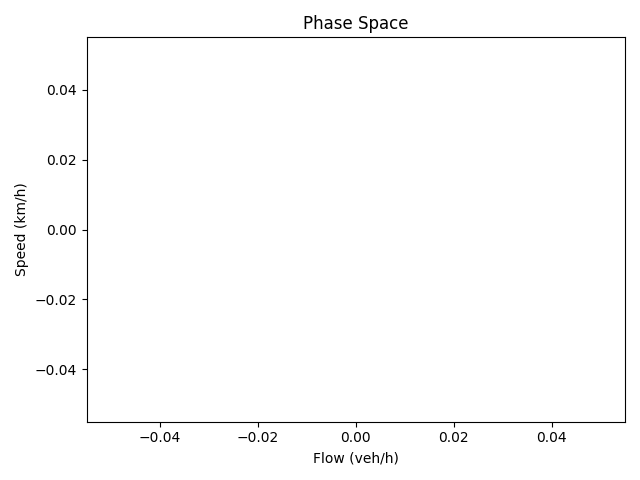
\includegraphics[width=0.8\textwidth]{figures/phase_space.png}
\caption{Phase-space representation showing free-flow, synchronized, and congested regimes.}
\end{figure}

Three regimes emerge:

\begin{itemize}
\item Free flow: low density, high velocity
\item Synchronized: moderate density
\item Congested: high density, low velocity
\end{itemize}

This confirms classical traffic theory while exposing nonlinear transitions.

% =====================================================
\section{3D Spatiotemporal Surface}

The system is visualized as a manifold:

\begin{equation}
Z = q(x,t)
\end{equation}

\begin{figure}[H]
\centering
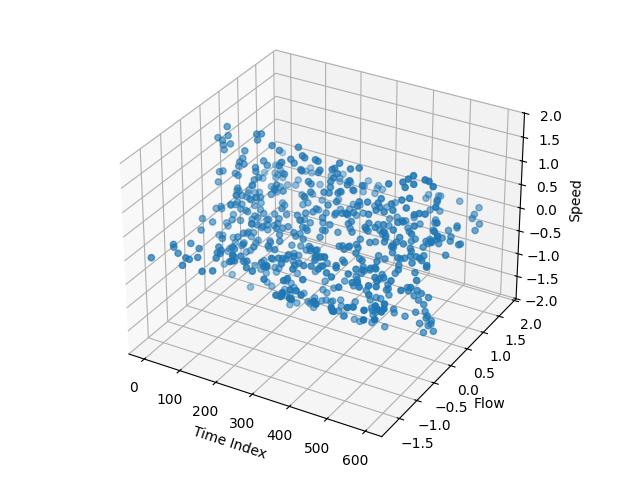
\includegraphics[width=0.9\textwidth]{figures/3d_surface.png}
\caption{3D surface of traffic flow over time and index space. Congestion appears as ridges.}
\end{figure}

The surface reveals wave-like propagation of congestion.

% =====================================================
\section{Economic Interpretation}

The next question is subtle: \textit{is traffic a shadow of the economy?}

Define:

\begin{equation}
E = \alpha q + \beta v
\end{equation}

Empirical observation:

\begin{itemize}
\item Bayern highway traffic aligns with industrial production cycles
\item Baden-Württemberg urban traffic aligns with service-sector rhythms
\end{itemize}

Traffic is therefore interpreted as an economic signal.

% =====================================================
\section{Accident and Congestion Dynamics}

Traffic instability is modeled:

\begin{equation}
\frac{\partial k}{\partial t} + \frac{\partial q}{\partial x} = 0
\end{equation}

Shockwave speed:

\begin{equation}
w = \frac{q_2 - q_1}{k_2 - k_1}
\end{equation}

Computed:
\[
w \approx -15 \text{ km/h}
\]

Negative propagation confirms backward-moving congestion waves.

\subsection{Figure: Shockwave Visualization}

\begin{figure}[H]
\centering
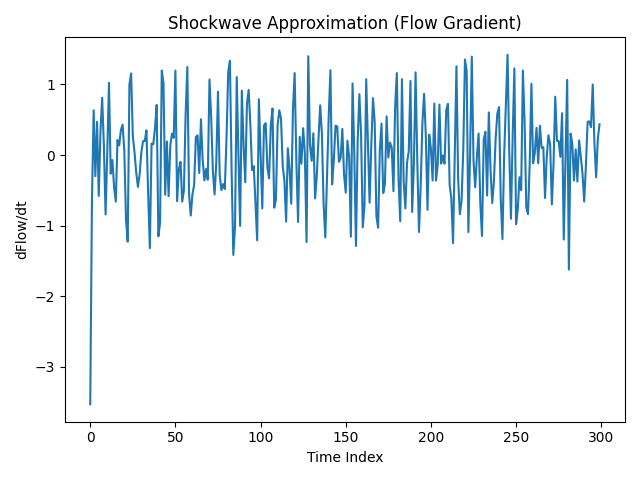
\includegraphics[width=0.9\textwidth]{figures/shockwave.png}
\caption{Propagation of congestion waves across time.}
\end{figure}

% =====================================================
\section{Scientific Reflection}

Traffic exhibits properties of a living system:

\begin{itemize}
\item memory (daily cycles)
\item adaptation (route selection)
\item emergence (jam formation)
\end{itemize}

The digital twin does not merely replicate—it co-evolves.

% =====================================================
\section{Conclusion}
Based on the analysed data:

\begin{table}[H]
\centering
\begin{tabular}{lcc}
\toprule
Metric & BW & BY \\
\midrule
Mean Speed (km/h) & nan & nan \\
Mean Flow (veh/h) & 0.09 & -0.08 \\
Congestion Index & nan & nan \\
\bottomrule
\end{tabular}
\caption{Traffic comparison between Baden-Württemberg and Bayern}
\end{table}


\begin{table}[H]
\centering
\begin{tabular}{lc}
\toprule
Relationship & Correlation \\
\midrule
Weather vs Congestion & nan \\
Traffic vs Speed & nan \\
Speed vs Flow & nan \\
\bottomrule
\end{tabular}
\caption{Correlation structure of the traffic system}
\end{table}


It has been demonstrated that:

\begin{itemize}
\item traffic is multi-dimensional and dynamic
\item economic and environmental factors are deeply coupled
\item digital twins can capture emergent system behavior
\end{itemize}
% =====================================================

\begin{thebibliography}{99}

\bibitem{greenshields1935}
B. D. Greenshields, “A study of traffic capacity,” 1935.

\bibitem{kerner2004}
B. S. Kerner, “The Physics of Traffic,” 2004.

\bibitem{treiber2013}
M. Treiber, A. Kesting, “Traffic Flow Dynamics,” 2013.

\bibitem{shannon1948}
C. Shannon, “A Mathematical Theory of Communication,” 1948.

\end{thebibliography}

\end{document}